\documentclass[conference,a4paper,10pt]{IEEEtran}
\IEEEoverridecommandlockouts

\usepackage{cite}
\usepackage{amsmath,amssymb,amsfonts}
\usepackage{graphicx}
\usepackage{textcomp}
\usepackage{xcolor}
\usepackage{booktabs}
\usepackage{tabularx}
\usepackage{array}
\usepackage{tikz}
\usepackage{url}
\usepackage{placeins}
\usepackage{fancyhdr}
\usepackage[hidelinks]{hyperref}
\usetikzlibrary{arrows.meta,calc,fit,positioning,decorations.pathreplacing}
\urlstyle{same}

% Keep the published IEEE text dimensions while closing gaps around wide figures.
\setlength{\dblfloatsep}{9pt plus 2pt minus 2pt}
\setlength{\dbltextfloatsep}{14pt plus 2pt minus 3pt}

% ICCIT camera-ready notices appear only on the title page.
\fancypagestyle{iccitfirstpage}{%
  \fancyhf{}%
  % Keep the two-line notice in the existing header area.
  \fancyhead[L]{\footnotesize\raisebox{0pt}[0pt][0pt]{\shortstack[l]{%
    2026 29th International Conference on Computer and Information Technology (ICCIT)\\
    18-20 December 2026, Cox's Bazar, Bangladesh}}}%
  \fancyfoot[L]{\footnotesize
    979-8-3195-0171-4/26/\$31.00~\copyright{}2026 IEEE}%
  \renewcommand{\headrulewidth}{0pt}%
  \renewcommand{\footrulewidth}{0pt}%
}
\pagestyle{empty}

\definecolor{jbblue}{RGB}{35,91,133}
\definecolor{jbteal}{RGB}{35,116,105}
\definecolor{jbamber}{RGB}{171,106,29}
\definecolor{jbred}{RGB}{158,48,48}
\definecolor{jbgray}{RGB}{241,243,245}
\definecolor{jbink}{RGB}{39,50,56}

\def\BibTeX{{\rm B\kern-.05em{\sc i\kern-.025em b}\kern-.08em
    T\kern-.1667em\lower.7ex\hbox{E}\kern-.125emX}}

\begin{document}

\title{Islands of Reach: A Censorship-Resistant Federated Forum for
National Internet Blackouts}

\author{%
  \IEEEauthorblockN{Tasmir Hossain Zihad\quad Sarwad Hasan Siddiqui\quad Rezuan Mustafa Hasan}
  \IEEEauthorblockA{Khulna University of Engineering \& Technology\\
    Khulna 9203, Bangladesh\\
    \texttt{tasmir@tuta.io}\quad \texttt{sarwad015@gmail.com}\quad
    \texttt{hasanideal2002@gmail.com}}
}

\maketitle
\thispagestyle{iccitfirstpage}

\begin{abstract}
A loss of international transit can leave domestic Internet paths available. We evaluate a federated forum that uses those paths to relay exact-byte signed posts, with verifiable admission receipts and caller-initiated recovery. On one Docker host, we published 20 certificate--community--post chains before withdrawing the direct exchange path and another 20 afterward. All 40 reached their destination. Median post latency was 0.735 seconds with the exchange intact and 1.732 seconds via the bridge after the cut. All 10 posts arrived in each of six network-emulation scenarios. A minimal ActivityPub push baseline and our prototype both delivered all 20 posts under a constrained lossy link. With inbound connections blocked, periodic pull recovered all 10 posts in our prototype and the push baseline delivered none. TypeScript, Rust, and Python agreed on 20,000 generated and mutated envelope cases. The results characterize partition recovery under surviving IP paths in the tested environment.
\end{abstract}

\begin{IEEEkeywords}
federated systems, Internet shutdowns, network partitions, signed objects, store-and-forward
\end{IEEEkeywords}

\section{Introduction}

Internet shutdowns can restrict bandwidth, block destinations or protocols, or withdraw international routes \cite{ooni2025bangladesh,bischof2023shutdowns}. Domestic networks may still exchange traffic. Baltra et al.~\cite{baltra2024connectivity} distinguish connectivity islands, whose members retain local reachability, from peninsulas with partial Internet reachability. We ask whether independently operated forum servers can accept signed posts locally and recover missing objects over the remaining IP paths.

Jagoo Bahee uses the same byte-preserving admission path for local and relayed objects. A caller can push new objects and pull missed objects through outbound connections, subject to peer quotas. An explicitly trusted dual-homed relay validates and stores each object it forwards. The networking contribution is recovery through an outbound connection to a known peer. The security contribution is a receipt that lets a client show which object an operator admitted, even after the operator stops serving it.

\section{Background and Research Gap}

ActivityPub delivers social activities to actor inboxes \cite{activitypub}. AT Protocol defines signed repository commits, and Nostr uses signed events and relays \cite{atproto,nostr}. These systems motivate separate choices about event encoding, delivery, and interoperability. Snowflake provides circumvention via temporary proxies \cite{bocovich2024snowflake}. Anix, Rangzen, and Moby use device-to-device paths for environments with limited or absent IP service \cite{kamali2025anix,lerner2016rangzen,pradeep2022moby}. We study server federation where domestic IP connectivity survives and applications must continue accepting writes during a partition. Temporary proxies require a reachable rendezvous and bridge, and the nearby-device systems address a different connectivity regime. Our design examines the intermediate case where servers remain reachable within islands but some routes between them have disappeared. The goal is to retain the author's bytes, apply the same validity checks to local and relayed objects, and make duplicate delivery idempotent.

Certificate Transparency supplies Merkle inclusion and consistency proofs \cite{rfc6962,rfc9162}. PeerReview and CoSi illustrate stronger accountability designs based on verifiable histories or independent witnesses \cite{haeberlen2007peerreview,syta2016cosi}. Our threat model includes malformed inputs, replay, and a server that later conceals an admitted object. A receipt provides evidence of admission. An operator that refuses a submission issues no receipt.

\section{System Design}

\subsection{Architecture and scheduling}

Clients submit envelopes over HTTP and nodes exchange them over gRPC (Fig.~\ref{fig:architecture}). A dual-homed bridge has an address on each island. Operators configure bridge trust in advance. Trust sets quota and traffic-class eligibility. The bridge repeats admission checks, stores accepted bytes, applies a quota keyed by source uplink, destination uplink, and priority, and excludes the sending peer from fan-out. The durable outbox drains in priority and sequence order, groups work by peer and plane, and uses concurrent peer leases so a stalled connection cannot serialize delivery across peers.

\begin{figure*}[!t]
  \centering
  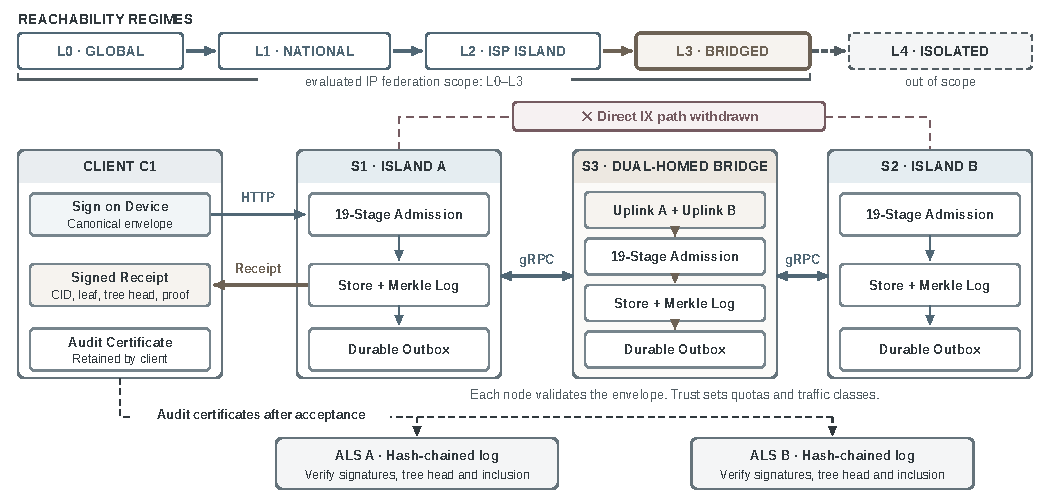
\includegraphics[width=\textwidth,trim=0 0 0 47bp,clip]{figures-v2/fig1-system-architecture-muted.pdf}
  \caption{Clients, validating nodes, dual-homed relay, and independent audit-log service (ALS). Solid links carry application or federation traffic. Audit certificates travel outside the admission path.}
  \label{fig:architecture}
\end{figure*}

\subsection{Signed objects and admission}

An envelope includes a domain, author key, nonce, creation timestamp, and payload. The receiver checks \texttt{created\_at\_ms} against a window from seven days before its clock to ten minutes after it. The author signs the canonical encoding with Ed25519 \cite{bernstein2012ed25519}. Since generic protobuf serialization can vary \cite{protobufnotcanonical}, each decoder requires the received bytes to match the canonical re-encoding. Federation preserves the signed bytes. The canonical profile uses ascending field order and minimal varints and rejects unknown fields. The SHA-256 content identifier binds the canonical bytes. If a relay re-encoded an incoming object before validation, it could hide a noncanonical wire representation by reconstructing the bytes the author signed. Receivers compare first and reject a mismatch before handling the payload.

HTTP rate limits and gRPC peer quotas precede the admission pipeline (Fig.~\ref{fig:pipeline}). Stages 1--12 perform read-only checks, including encoding, signature, certificate, and replay checks. Stage 13 applies origin anti-abuse policy, stage 14 authorizes the operation, and stage 15 checks its semantics. The commit stores the envelope and projection and appends a Merkle leaf. An idempotent repeat returns the existing receipt. Reuse of a spent nonce on a non-idempotent operation yields a replay rejection. A database uniqueness constraint handles identical deliveries racing through push and backfill. Origin anti-abuse charges apply once, at the originating node. The receiving peer still checks the object's validity and enforces its own federation quota.

\begin{figure}[!t]
  \centering
  {\normalsize
  \begin{tabularx}{\columnwidth}{@{}l>{\raggedright\arraybackslash}X@{}}
    \toprule
    \textbf{Stage} & \textbf{Check or action} \\
    \midrule
    Before stage 1 & HTTP rate limit or gRPC peer quota \\
    \midrule
    1--2 & Size, parse, canonical re-encoding \\
    3--7 & Version, domain, plane, size, algorithm, priority \\
    8--10 & Clock window, signature, certificate \\
    11--12 & Content-ID deduplication and nonce replay check \\
    \midrule
    13 & Origin anti-abuse policy \\
    14--15 & Authorization and semantic validation \\
    16--18 & Atomic storage, projection, Merkle append, and signed receipt \\
    19 & Durable fan-out to eligible peers \\
    \bottomrule
  \end{tabularx}}
  \caption{Admission pipeline for local and federated envelopes. Entry quotas precede the read-only checks and authorization occurs at stage 14.}
  \label{fig:pipeline}
\end{figure}

\subsection{Partition-aware federation}

\textsc{Deliver} pushes batches to known peers. \textsc{StreamActivities} reads a finite snapshot from a cursor, and \textsc{Backfill} supplies missed entries. A timer checks for catch-up every 2\,s by default. Outbound-only nodes poll known peers. Other nodes initiate catch-up when inbound activity is stale, with a threshold of two polling intervals. In the route-cut topology (Fig.~\ref{fig:topology}), the bridge carries traffic between the islands after the exchange path disappears.

Delivery has a 15\,s default deadline and propagates cancellation to the gRPC call through an abort signal. Control calls default to 5\,s and backfill to 30\,s. Retry delays double from 1\,s to a 15\,min cap, with dead-lettering on the 13th failure. The backoff delays sum to 47\,min 3\,s before that attempt, excluding RPC time and scheduling. Peer backpressure hints are capped at 60\,s. The testbed probes uplinks every 5\,s with a 1.5\,s timeout and a two-failure threshold. On the rebuilt image the ISP gate passed 22 of 22 criteria in 39.91\,s.

\begin{figure}[!t]
  \centering
  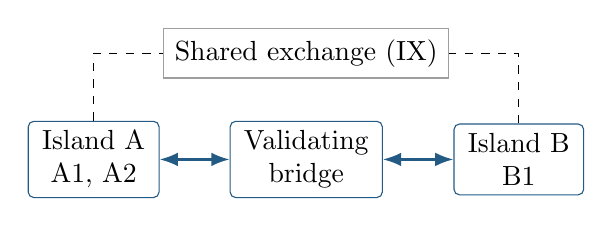
\begin{tikzpicture}[font=\normalsize,>=Latex,role/.style={draw=jbblue,rounded corners=2pt,align=center,minimum height=9mm,inner xsep=5pt}]
    \node[role] (a) at (0,0) {Island A\\A1, A2};
    \node[role] (r) at (2.7,0) {Validating\\bridge};
    \node[role] (b) at (5.4,0) {Island B\\B1};
    \node[draw=jbgray!65!black,align=center,inner sep=4pt] (ix) at (2.7,1.35) {Shared exchange (IX)};
    \draw[<->,thick,jbblue] (a) -- (r);
    \draw[<->,thick,jbblue] (r) -- (b);
    \draw[dashed] (a.north) |- (ix.west);
    \draw[dashed] (b.north) |- (ix.east);
  \end{tikzpicture}
  \caption{Four-node route-cut testbed. Withdrawing the dashed exchange path leaves A1 and B1 connected through the dual-homed bridge. A2 remains on island A.}
  \label{fig:topology}
\end{figure}

\subsection{Audit guarantees}

An independent ALS can retain a client's audit certificate in a hash-chained store. Before appending, it checks canonical envelope decoding, the author signature, the content and server identifiers, the server receipt signature, and the signed tree head (STH) and inclusion proof carried with the receipt. Table~\ref{tab:audit} describes the scope of verification. The receipt binds the content identifier and Merkle leaf position, so a client that retains it can show what the server accepted even if the server later hides the object. The peer comparison first checks that the head names the expected server key and discards observations that predate the recorded head. It then compares tree size and root. This check does not independently verify the head signature. A larger head advances the stored observation without proving append-only growth.

\begin{table}[!t]
  \caption{Audit Verification and Its Boundaries}
  \label{tab:audit}
  \centering
  \begin{tabularx}{\columnwidth}{@{}p{.22\columnwidth}X@{}}
    \toprule
    Scope & Guarantee \\
    \midrule
    Admission & Signed receipts and inclusion proofs give evidence for specific accepted bytes. The ALS verifies and retains certificates independently. \\
    Log growth & Local RFC 6962 consistency proof generation and verification are implemented, with proof retrieval over HTTP. Peer gRPC exchange does not verify growing heads for append-only consistency. \\
    Peer heads & Among non-stale heads naming the expected key, a peer flags a different root at the same size or a smaller tree. Split views across isolated observers and automated ALS cross-head auditing remain open. \\
    Refusal & Refusal before admission produces no receipt. \\
    \bottomrule
  \end{tabularx}
\end{table}

\section{Methodology}

The controlled network and load experiments used Docker virtual networks on one physical host. The route-cut, impairment, stress, and scaling datasets precede the final rebuild that introduced bounded gRPC calls and steady-state pull. The ISP gate and controlled ActivityPub and blocked-inbound runs use the rebuilt image. We treat these datasets as separate measurements of their respective builds.

\begin{figure*}[!t]
  \centering
  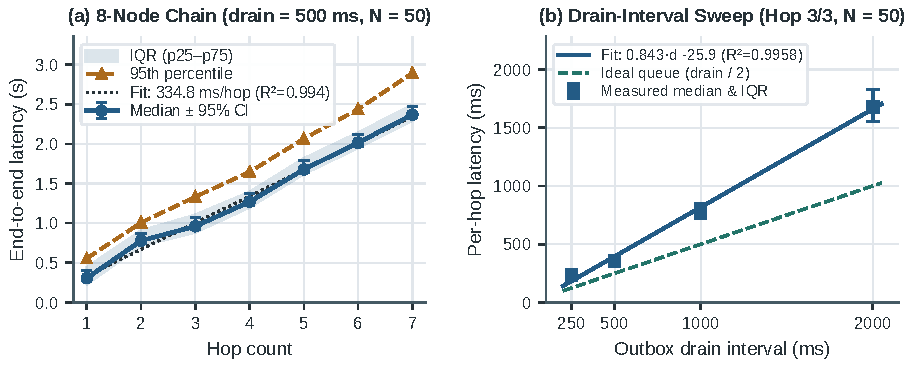
\includegraphics[width=\textwidth]{figures-v2/fig4-hop-and-drain-scaling.pdf}
  \caption{Hop and drain-interval scaling, 50 posts per configuration. The left panel uses an eight-node chain and a 500\,ms drain interval. The right panel divides the median latency to hop three by three. Its dashed line shows half the configured drain interval.}
  \label{fig:chain}
\end{figure*}

\begin{figure*}[!t]
  \centering
  \begin{minipage}[t]{.45\textwidth}
    \centering\textbf{(a) Route regimes, 20 chains each}\\[3pt]
    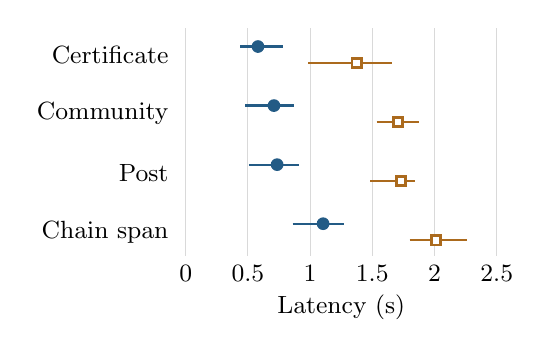
\begin{tikzpicture}[x=1.58cm,y=.75cm,font=\small]
      \foreach \x in {0,.5,1,1.5,2,2.5} {
        \draw[gray!30] (\x,.60) -- (\x,4.45);
        \node[below] at (\x,.6) {\pgfmathprintnumber{\x}};
      }
      \foreach \y/\labeltext in {4/Certificate,3/Community,2/Post,1/Chain span}
        \node[anchor=east] at (-.06,\y) {\labeltext};
      \foreach \y/\m/\lo/\hi in {4/.581/.4395/.7815,3/.7095/.479/.874,2/.735/.507/.9125,1/1.1045/.8595/1.2755} {
        \draw[jbblue,thick] (\lo,\y+.14) -- (\hi,\y+.14);
        \fill[jbblue] (\m,\y+.14) circle[radius=2.3pt];
      }
      \foreach \y/\m/\lo/\hi in {4/1.3745/.9855/1.6575,3/1.7065/1.534/1.879,2/1.7315/1.4815/1.841,1/2.013/1.7995/2.2575} {
        \draw[jbamber,thick] (\lo,\y-.14) -- (\hi,\y-.14);
        \node[rectangle,draw=jbamber,fill=white,inner sep=1.65pt,line width=.9pt] at (\m,\y-.14) {};
      }
      \node[below] at (1.25,.10) {Latency (s)};
    \end{tikzpicture}
  \end{minipage}\hfill
  \begin{minipage}[t]{.54\textwidth}
    \centering\textbf{(b) Bridge egress, 10 posts per condition}\\[3pt]
    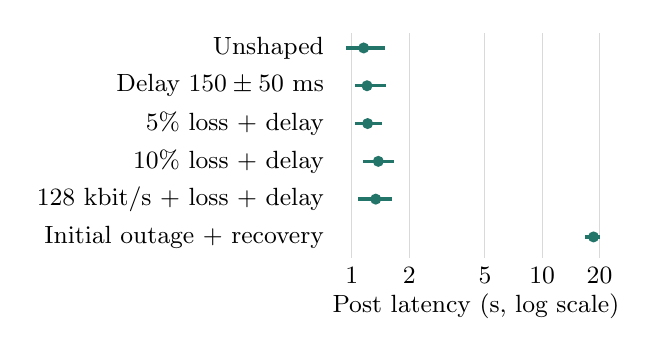
\begin{tikzpicture}[x=1.05cm,y=.48cm,font=\small]
      \foreach \x in {1,2,5,10,20} {
        \draw[gray!30] ({ln(\x)},.45) -- ({ln(\x)},6.4);
        \node[below] at ({ln(\x)},.45) {\x};
      }
      \foreach \y/\labeltext/\m/\lo/\hi in {
        6/Unshaped/1.1535/.929/1.491,
        5/{Delay $150\pm50$ ms}/1.2015/1.0395/1.507,
        4/{5\% loss + delay}/1.210/1.0405/1.448,
        3/{10\% loss + delay}/1.377/1.145/1.665,
        2/{128 kbit/s + loss + delay}/1.335/1.0785/1.623,
        1/Initial outage + recovery/18.595/16.841/20.071} {
        \node[anchor=east] at (-.22,\y) {\labeltext};
        \draw[jbteal,very thick] ({ln(\lo)},\y) -- ({ln(\hi)},\y);
        \fill[jbteal] ({ln(\m)},\y) circle[radius=2.0pt];
      }
      \node[below] at (1.5,-.25) {Post latency (s, log scale)};
    \end{tikzpicture}
  \end{minipage}
  \caption{Median latency and 95\% bootstrap intervals. In (a), filled circles mark the intact exchange and open squares the bridged route. In (b), all 10 posts arrived under each condition. Delay is configured egress delay. The interruption batch was queued before the first recovery.}
  \label{fig:netem}
\end{figure*}

The ISP gate checked established sockets in the bridge container's kernel TCP tables for both configured source IP addresses. The gate then disconnected the exchange links, confirmed that A1 could no longer resolve B1 on the direct network, and confirmed that B1 lacked the crossing post before A1 published it. It checked for the exact post ID at B1 and checked the bridge's cross-uplink relay counters. Other gate checks covered reserved capacity and the loss and recovery of one bridge uplink. The gate verified reachability by polling. The repeated-trial latency estimates below use insertion timestamps instead.

We published 20 chains with the exchange intact, withdrew the direct path once, and published 20 more on the same stack. Each chain used a fresh identity and community. Latencies subtract source from destination \texttt{received\_at\_ms}, using the shared host clock. Chain span measures source certificate insertion to destination post insertion. We report sample counts and interquartile ranges (IQRs). For each median, a 95\% percentile bootstrap interval uses 10,000 resamples within the regime. These intervals describe within-run variation. For impairment tests we shaped bridge federation traffic on TCP port 8444, leaving database traffic unshaped. The unshaped control and five impairment scenarios each used ten posts. The scaling runs used 50 posts per configuration, an eight-node chain at a 500\,ms drain interval, and a four-node sweep at 250, 500, 1,000, and 2,000\,ms. Each post follows the same linear path, so successive hops observe the same posts. Each node has its own logical database on a shared MongoDB process, so the measurements include contention on that process.

The stress experiments exercised HTTP admission, replay, federation peer quotas, and single-node valid writes. We recorded response codes, latency, database collection deltas, and MongoDB profiler counts where instrumented. CPU and memory values come from Docker snapshots. The concurrent-write workload uses 32 certified identities and 200 posts at each concurrency setting.

The ActivityPub comparison pairs two Jagoo Bahee nodes with two minimal Node.js inbox peers implementing gzip, HTTP signatures, and push retries. Both pairs use the same shaping settings on WAN interfaces separate from the databases. The WAN shaping adds 75\,ms delay per direction with 15\,ms variation, 5\% loss, and a 128\,kbit/s cap. We measured transmit bytes on each sender's WAN interface over its run. This includes framing and can include background traffic. Jagoo Bahee measures the interval between source and destination envelope insertion timestamps. The inbox times from the sender's delivery routine, before compression and signing, to the receiver's verified and decoded activity, which it records in memory. Separately, we sampled 40 public Mastodon \texttt{Create}/\texttt{Note} activities from fosstodon.org. For each activity, we restored the host's JSON-LD context and measured the raw and gzipped JSON representations. Non-text overhead subtracts the authored UTF-8 text from the raw representation.

\begin{table*}[!t]
  \caption{Admission under load. Memory was sampled after each valid-write batch.}
  \label{tab:stress}
  \centering
  \begingroup
  \small
  \setlength{\tabcolsep}{3pt}
  \renewcommand{\arraystretch}{1.12}
  \begin{minipage}[t]{.49\textwidth}
    \textbf{(a) HTTP admission at concurrency 16}\par\smallskip
    \begin{tabular*}{\linewidth}{@{}l@{\extracolsep{\fill}}rr@{}}
      \toprule
      Request batch & Requests/s & Median (ms) \\
      \midrule
      Invalid input, default HTTP limit & 1,347 & 6.01 \\
      Invalid input, raised HTTP limit & 293 & 55.31 \\
      Malformed protobuf & 2,383 & 5.87 \\
      Exact duplicate & 159 & 92.45 \\
      Reused nonce & 134 & 116.06 \\
      \bottomrule
    \end{tabular*}
  \end{minipage}\hfill
  \begin{minipage}[t]{.48\textwidth}
    \textbf{(b) Valid writes, 200 posts total per setting}\par\smallskip
    \begin{tabular*}{\linewidth}{@{}r@{\extracolsep{\fill}}rrrr@{}}
      \toprule
      & & \multicolumn{2}{c}{Latency (ms)} & Node memory \\
      Concurrency & Requests/s & Median & p95 & (MiB) \\
      \midrule
      1  & 29 & 32.06    & 49.41     & 108 \\
      4  & 27 & 104.33   & 352.60    & 133 \\
      16 & 9  & 1,300.69 & 4,132.36  & 175 \\
      32 & 6  & 4,192.33 & 12,586.59 & 181 \\
      \bottomrule
    \end{tabular*}
  \end{minipage}
  \endgroup
\end{table*}

\begin{table*}[!t]
  \caption{Object sizes, delivery latency, and sender-interface traffic. The shaped link used 128\,kbit/s, 5\% loss, and 75\,ms added delay per direction.}
  \label{tab:ap}
  \centering
  \begingroup
  \small
  \setlength{\tabcolsep}{3pt}
  \renewcommand{\arraystretch}{1.12}
  \begin{minipage}[t]{.49\textwidth}
    \textbf{(a) Object representations (bytes)}\par\smallskip
    \begin{tabular*}{\linewidth}{@{}l@{\extracolsep{\fill}}rrr@{}}
      \toprule
      Source & Full raw & Non-text raw & Full gzip \\
      \midrule
      Mastodon (40 activities) & 3,931 & 3,627 & 1,063 \\
      \addlinespace[2pt]
      Jagoo Bahee check-in & 155 & 155 & --- \\
      Jagoo Bahee broadcast & 243 & 177 & --- \\
      Jagoo Bahee post & 220 & 206 & --- \\
      \bottomrule
    \end{tabular*}
  \end{minipage}\hfill
  \begin{minipage}[t]{.48\textwidth}
    \textbf{(b) Delivery under asymmetric reachability}\par\smallskip
    \begin{tabular*}{\linewidth}{@{}l@{\extracolsep{\fill}}rr@{}}
      \toprule
      Delivery method & Delivered & Median (ms) \\
      \midrule
      \multicolumn{3}{@{}l}{\emph{Inbound federation traffic blocked}} \\
      Jagoo Bahee periodic pull & 10/10 & 1,045.5 \\
      Minimal inbox push & 0/10 & --- \\
      \multicolumn{3}{@{}l}{\emph{Jagoo Bahee with listener disabled}} \\
      Backfill from startup & 10/10 & 4,957 \\
      Outbound push & 10/10 & 340.5 \\
      \bottomrule
    \end{tabular*}
  \end{minipage}

  \smallskip
  \begin{minipage}{\textwidth}
    \textbf{(c) Delivery on the shaped link}\par\smallskip
    \begin{tabular*}{\linewidth}{@{}l@{\extracolsep{\fill}}lrrr@{}}
      \toprule
      System & Timed interval & Delivered & Median (ms) & Sender interface (B/post) \\
      \midrule
      Jagoo Bahee & Origin insertion to destination insertion & 20/20 & 520.5 & 1,846.4 \\
      Minimal inbox & Sender delivery routine to in-memory receipt & 20/20 & 154.5 & 1,278.3 \\
      \bottomrule
    \end{tabular*}
  \end{minipage}
  \endgroup
\end{table*}

\section{Results}

\subsection{Decoding, route cuts, and impairment}

TypeScript, Rust, and Python agreed on 16 canonical reference vectors and 20,000 seeded differential cases. All three matched on bytes, content identifiers, and round-trip decoding for 10,000 generated wire-format cases, including numeric boundaries, NFC Unicode, and empty anti-abuse fields. Across 16 mutation classes, all three decoders rejected 9,455 inputs and decoded the same 545. These tests measure encoding agreement and do not exercise signature verification or application admission. An earlier pass exposed a TypeScript unsigned 32-bit bounds error, which was corrected and covered by a regression test.

The destination received 20 of 20 certificates, communities, and posts in each route regime (Figs.~\ref{fig:topology} and \ref{fig:netem}). Post median latency rose from 735\,ms (IQR 436\,ms, 95\% CI 507--913\,ms) to 1,732\,ms (IQR 446\,ms, CI 1,482--1,841\,ms). Sample standard deviations were 260 and 298\,ms. Certificate and community medians were 581 and 710\,ms with the exchange intact (CIs 440--782 and 479--874\,ms) and 1,375 and 1,707\,ms via the bridge (CIs 986--1,658 and 1,534--1,879\,ms). Median chain span rose from 1,105 to 2,013\,ms (bridged CI 1,800--2,258\,ms). All six emulation scenarios delivered 10 of 10 posts. Median post latency was 1.154\,s with no shaping, 1.202\,s with 150\,ms delay and 50\,ms variation, 1.210 and 1.377\,s at 5\% and 10\% loss with added delay, and 1.335\,s at 128\,kbit/s with delay and 2\% loss. For the interruption test, all ten posts were submitted during full loss on the bridge's island-B uplink. The harness waited another 8\,s after the batch finished before restoring the link. Two further loss/recovery cycles used 8\,s per phase. Median latency for the initially queued posts was 18.595\,s (CI 16.841--20.071\,s).

\subsection{Scaling, stress, and resource use}

The eight-node chain delivered 50 of 50 posts at each hop. At hop seven, the median was 2.368\,s (CI 2.332--2.469\,s, IQR 0.191\,s, p95 2.893\,s). The fitted median slope was 335\,ms per hop ($R^2=0.994$). At hop three in the drain sweep, medians were 0.707, 1.067, 2.365, and 5.035\,s, with 50 of 50 deliveries in each configuration. Median hop-three latency divided by three increased by 0.843\,ms per millisecond of drain interval ($R^2=0.996$). The repeated 500\,ms control shifted by 10.9\% between the first and final runs. The original 200-envelope run used a 1,000\,ms drain interval and reached hop seven with a 4.125\,s median and 6.115\,s p99. Its different drain interval and workload place it outside the 50-post sweep.

The HTTP limiter rejected 2,709 of 3,000 requests in the default invalid-input run. With that limit raised, 2,593 of 3,000 reached bad-signature rejection and the batch processed 293 requests/s. The malformed-protobuf batch returned 3,000 HTTP 400 responses and zero HTTP 500 responses. Exact repeats returned 1,000 existing receipts. A separate non-idempotent nonce-reuse run returned 1,000 replay rejections. These batches produced zero profiled database writes. Across five gRPC peers, the receiver rejected all 500 invalid-signature frames. In over-quota rounds it blocked two peers, recorded 15 peer-state writes, and admitted no envelopes.

All 200 valid posts per setting reached the single-node projection. At concurrency 1, 4, 16, and 32, throughput was 29, 27, 9, and 6 requests/s, with p95 latencies of 49, 353, 4,132, and 12,587\,ms (Table~\ref{tab:stress}). The p99 rose from 60\,ms to 15.940\,s. Docker memory snapshots for the node were 87\,MiB idle and 108--181\,MiB after the valid-write batches. Corresponding MongoDB snapshots ranged from 150 to 345\,MiB and Redis remained below 9.5\,MiB. At eight nodes the application containers used 77--111\,MiB each, with a sampled CPU maximum of 21.18\%. The shared MongoDB and Redis containers used 184 and 9\,MiB. The route-cut snapshots recorded 105--151\,MiB of memory and 0.59--30.72\% CPU across active application containers.

\subsection{ActivityPub and blocked-inbound delivery}

Both systems delivered 20 of 20 posts over the constrained lossy link (Table~\ref{tab:ap}). Jagoo Bahee had a median of 521\,ms (CI 394--586\,ms) and 1,846 sender-interface bytes per post. The minimal AP inbox had a median of 155\,ms (CI 145--161\,ms) and 1,278 sender-interface bytes per post. The application containers used 88--92\,MiB for Jagoo Bahee and 9--14\,MiB for the inbox baseline. This baseline implements a small HTTP inbox with retries and omits Mastodon's application and worker stack.

In a separate run with shaping removed and inbound federation ports blocked, none of ten inbox pushes succeeded within the baseline's retry budget. Jagoo Bahee's periodic pull recovered ten of ten (median 1.046\,s, CI 0.469--1.509\,s). In a separate run with the federation listener disabled, an outbound-only node recovered 10 of 10 existing posts (median 4.957\,s from startup) and pushed 10 of 10 new posts (median 0.341\,s).

The original 80-activity sample from two deployments had a gzipped median of 1,074\,B. The later 40-activity sample from one deployment had median full representations of 3,931\,B raw and 1,063\,B gzipped. Median non-text overhead was 3,627\,B. Example Jagoo Bahee signed objects have 155, 177, and 206\,B of non-text data for a check-in, a Bangla broadcast, and a forum post. The sizes reflect extensible JSON-LD activities and a fixed canonical protobuf schema with different features and interoperability. Sender-interface measurements include transport effects that object sizes omit. Rejecting unknown fields keeps signature verification tied to a defined schema, but version changes require coordinated decoder support. JSON-LD allows vocabulary extension and carries interoperability across existing Fediverse deployments. The controlled inbox comparison measures one delivery workload rather than those compatibility costs.

\section{Discussion and Limitations}

The controlled experiments share one host kernel, clock, CPU, and storage system. Because the intact trials always ran first, we cannot separate the effect of route condition from changes in host load over time. The shared clock supports subtraction of insertion timestamps within this testbed. An independent-host replication would place the two islands and bridge on separate machines, repeat the withdrawal, and record clock offsets before comparing insertion times. Real routing, failures across independent machines, variable access links, and wide-area latency remain unmeasured. The CPU and memory snapshots characterize the tested x86 setup. Peak resident memory, disk footprint, and sustained resource-exhaustion thresholds remain unmeasured. Deployment on a single-board computer requires measurements on that hardware.

Federation requires a surviving IP path and a known peer address. Subscriber isolation or complete loss of domestic routes limits operation to each local server. Source binding selects an uplink and leaves endpoints and timing visible to a network operator. Protocol whitelisting can block the gRPC traffic even while domestic routing continues. Signatures attest control of the signing key, and receipts preserve evidence of admissions. A permissive origin can admit large volumes of valid objects under its own policy, leaving remote peers dependent on their ingress quotas. Key theft, revocation recovery, moderation, and isolated split views are outside the measured guarantees.

We used synthetic content in the controlled trials and public activities for the encoding sample. Real deployments can expose bridge operators and participants to identification or pressure. They require local threat assessment, data minimization, and informed consent.

\section{Conclusion}

On the single-host Docker testbed, a validating bridge delivered dependent signed objects after withdrawal of the direct exchange route. Caller-initiated recovery delivered queued posts under the tested blocked-inbound conditions. Observed throughput declined as valid-write concurrency rose, and the minimal ActivityPub inbox transferred fewer sender-interface bytes per post on the tested lossy link. Independent multi-host trials, dedicated resource-exhaustion tests, and peer verification of growing logs remain open.

\section*{Disclosure}
The authors used OpenAI Codex to compare manuscript drafts, edit the manuscript and reviewer response, and revise figures and tables using previously reported measurements.

\IEEEtriggeratref{2}
\bibliographystyle{IEEEtran}
\bibliography{iccit2026-paper-pre-references}

\end{document}
